% Base template source: https://tex.stackexchange.com/questions/8827/preparing-cheat-sheets

\documentclass[10pt,landscape]{article}

\usepackage{multicol}
\usepackage{lipsum}

\usepackage{calc, ifthen,hyperref, gensymb, comment, textcomp}

\usepackage{amsmath,amsthm,amsfonts,amssymb}

\usepackage{color,graphicx,overpic}

\usepackage{geometry}
% This sets page margins to .5 inch if using letter paper, and to 1cm
% if using A4 paper. (This probably isn't strictly necessary.)
% If using another size paper, use default 1cm margins.
\ifthenelse{\lengthtest { \paperwidth = 11in}}
    { \geometry{top=.25in,left=.25in,right=.25in,bottom=.25in} }
    {\ifthenelse{ \lengthtest{ \paperwidth = 297mm}}
        {\geometry{top=1cm,left=1cm,right=1cm,bottom=1cm} }
        {\geometry{top=1cm,left=1cm,right=1cm,bottom=1cm} }
    }

% Turn off header and footer
\pagestyle{empty}

% Don't print section numbers
\setcounter{secnumdepth}{0}

% Define Image
\newenvironment{Figure}
     {\par\medskip\noindent\minipage{\linewidth}}
     {\endminipage\par\medskip}
    
% Define Line Spacing
\linespread{.3}
% -----------------------------------------------------------------------

\begin{document}
\raggedright
\footnotesize

% Area Above Columns
\begin{center}
     \Large{\underline{Solid Mechanics - Zak Olech - 9/10/2019}}
\end{center}
\begin{multicols}{3}

% multicol parameters
% These lengths are set only within the two main columns
\setlength{\columnseprule}{0.25pt}
\setlength{\premulticols}{1pt}
\setlength{\postmulticols}{1pt}
\setlength{\multicolsep}{1pt}
\setlength{\columnsep}{2pt}

\section{Variables (Alphbetical By Variable)}
\begin{Figure}
    \centering
    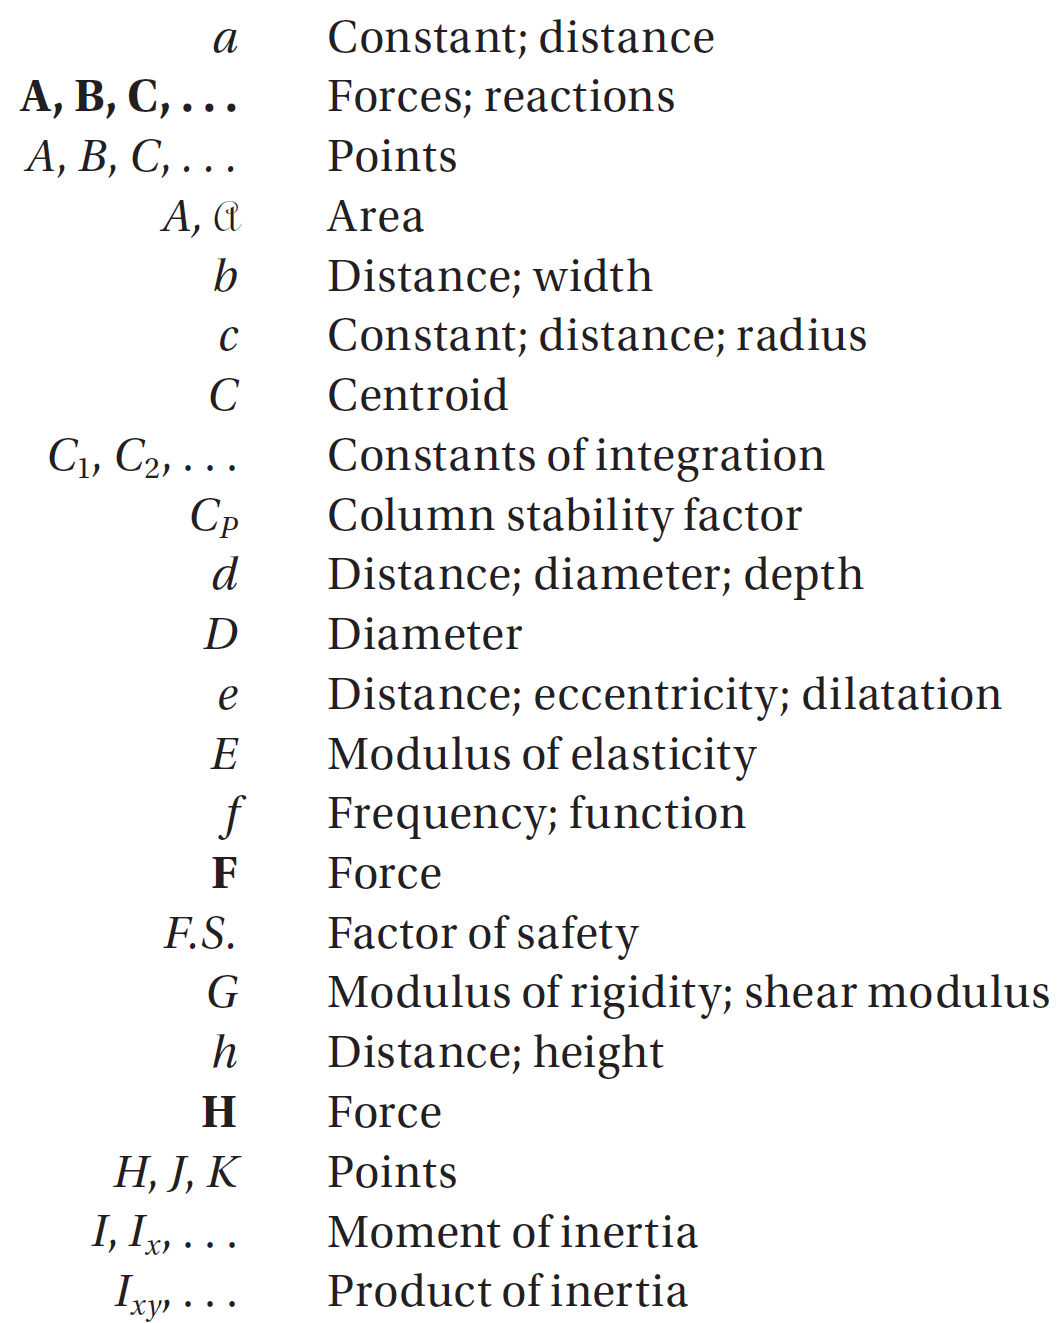
\includegraphics[width=\linewidth, height=8cm]{ListOfSymbols_Part_1.png}
\end{Figure}
\begin{Figure}
    \centering
    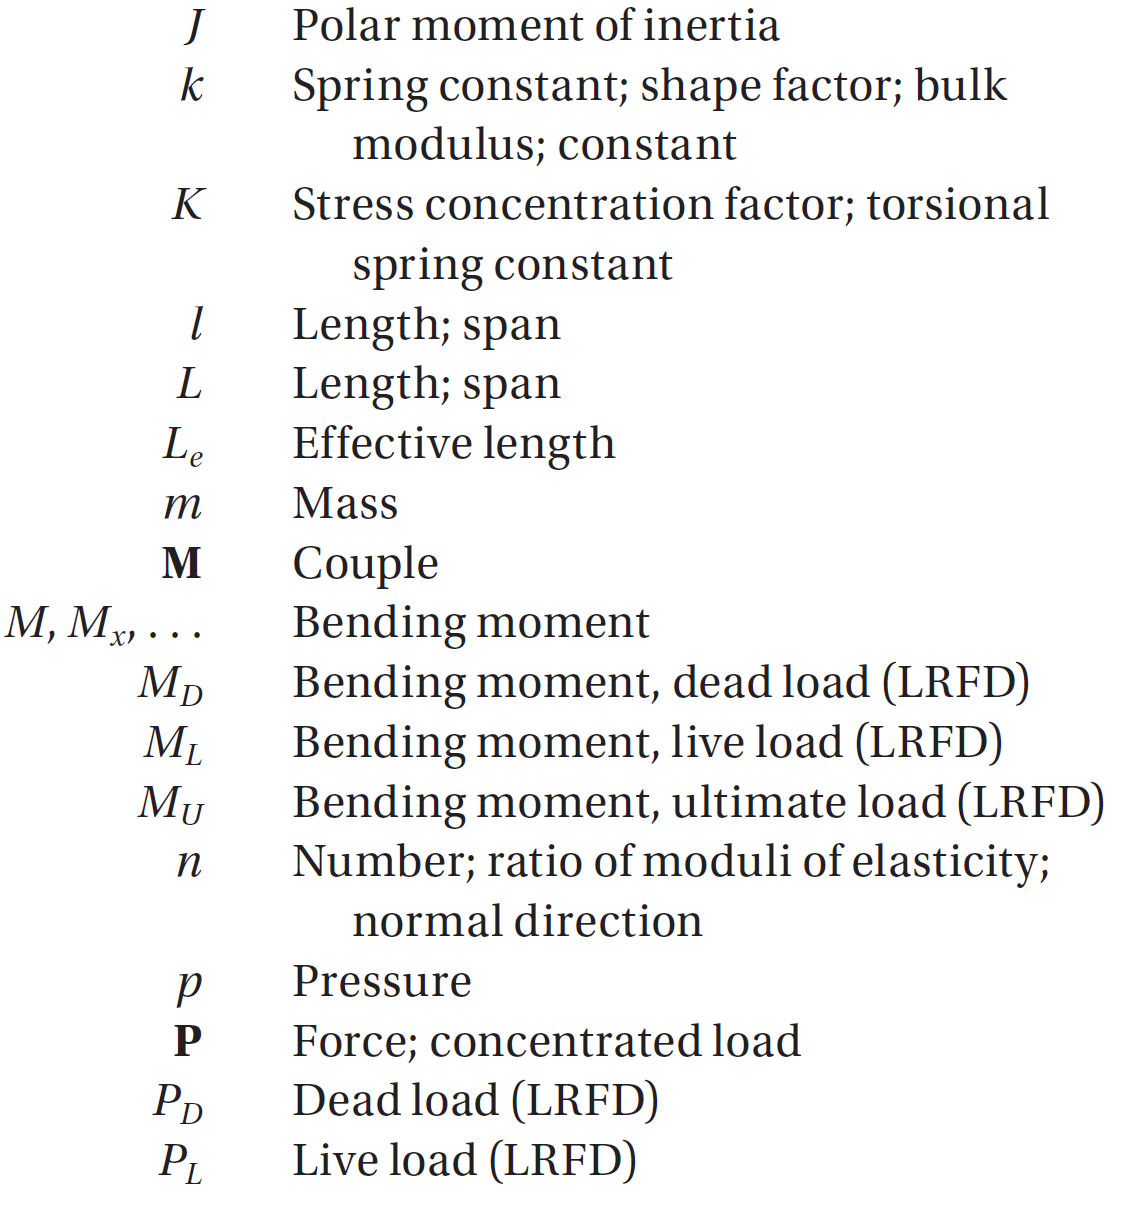
\includegraphics[width=\linewidth, height=8cm]{ListOfSymbols_Part_2.png}
\end{Figure}
\begin{Figure}
    \centering
    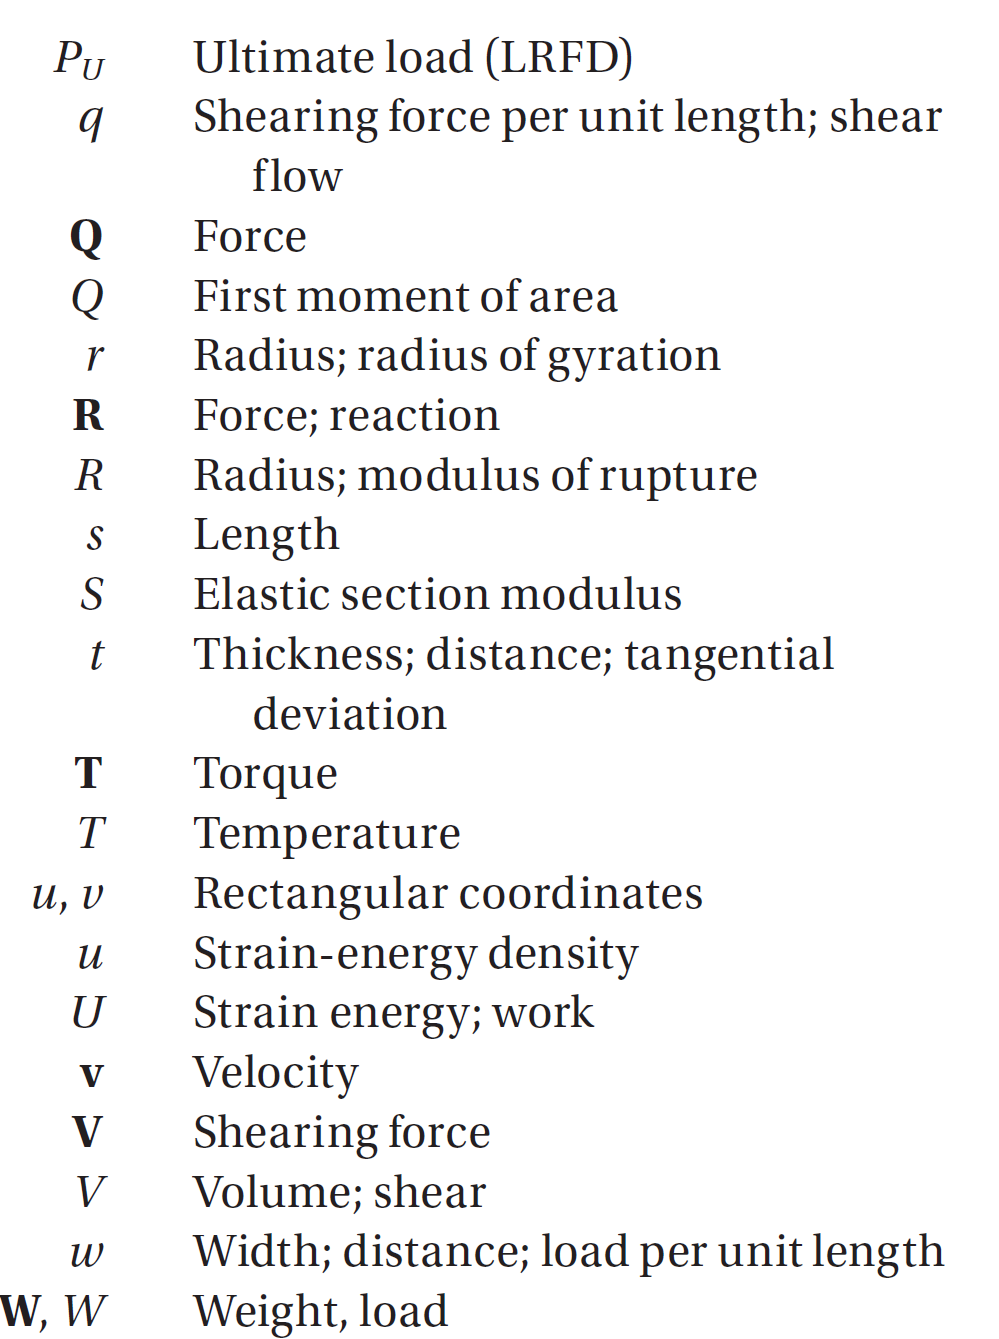
\includegraphics[width=\linewidth, height=8cm]{ListOfSymbols_Part_3.png}
\end{Figure}
\begin{Figure}
    \centering
    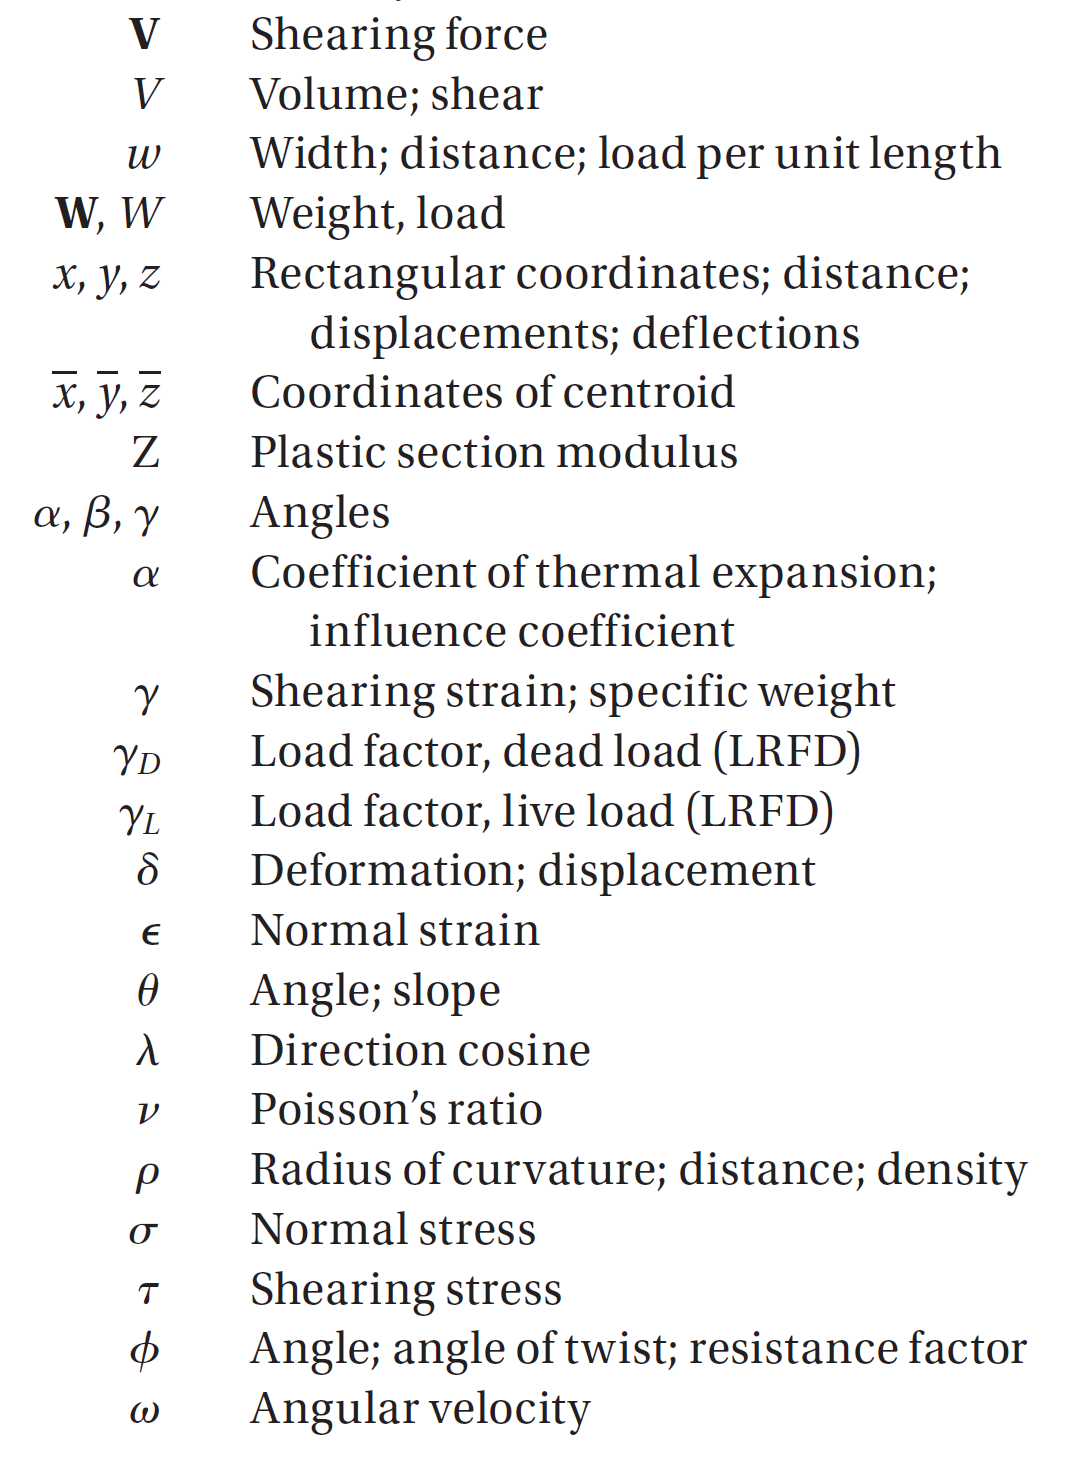
\includegraphics[width=\linewidth, height=10cm]{ListOfSymbols_Part_4.png}
\end{Figure}

\section{Conversion Factors}
\begin{equation}
    1\text{hp}=550\text{ft*lb/s}=6600\text{ in*lb/s}
\end{equation}

\section{General}
\begin{Figure}
    \centering
    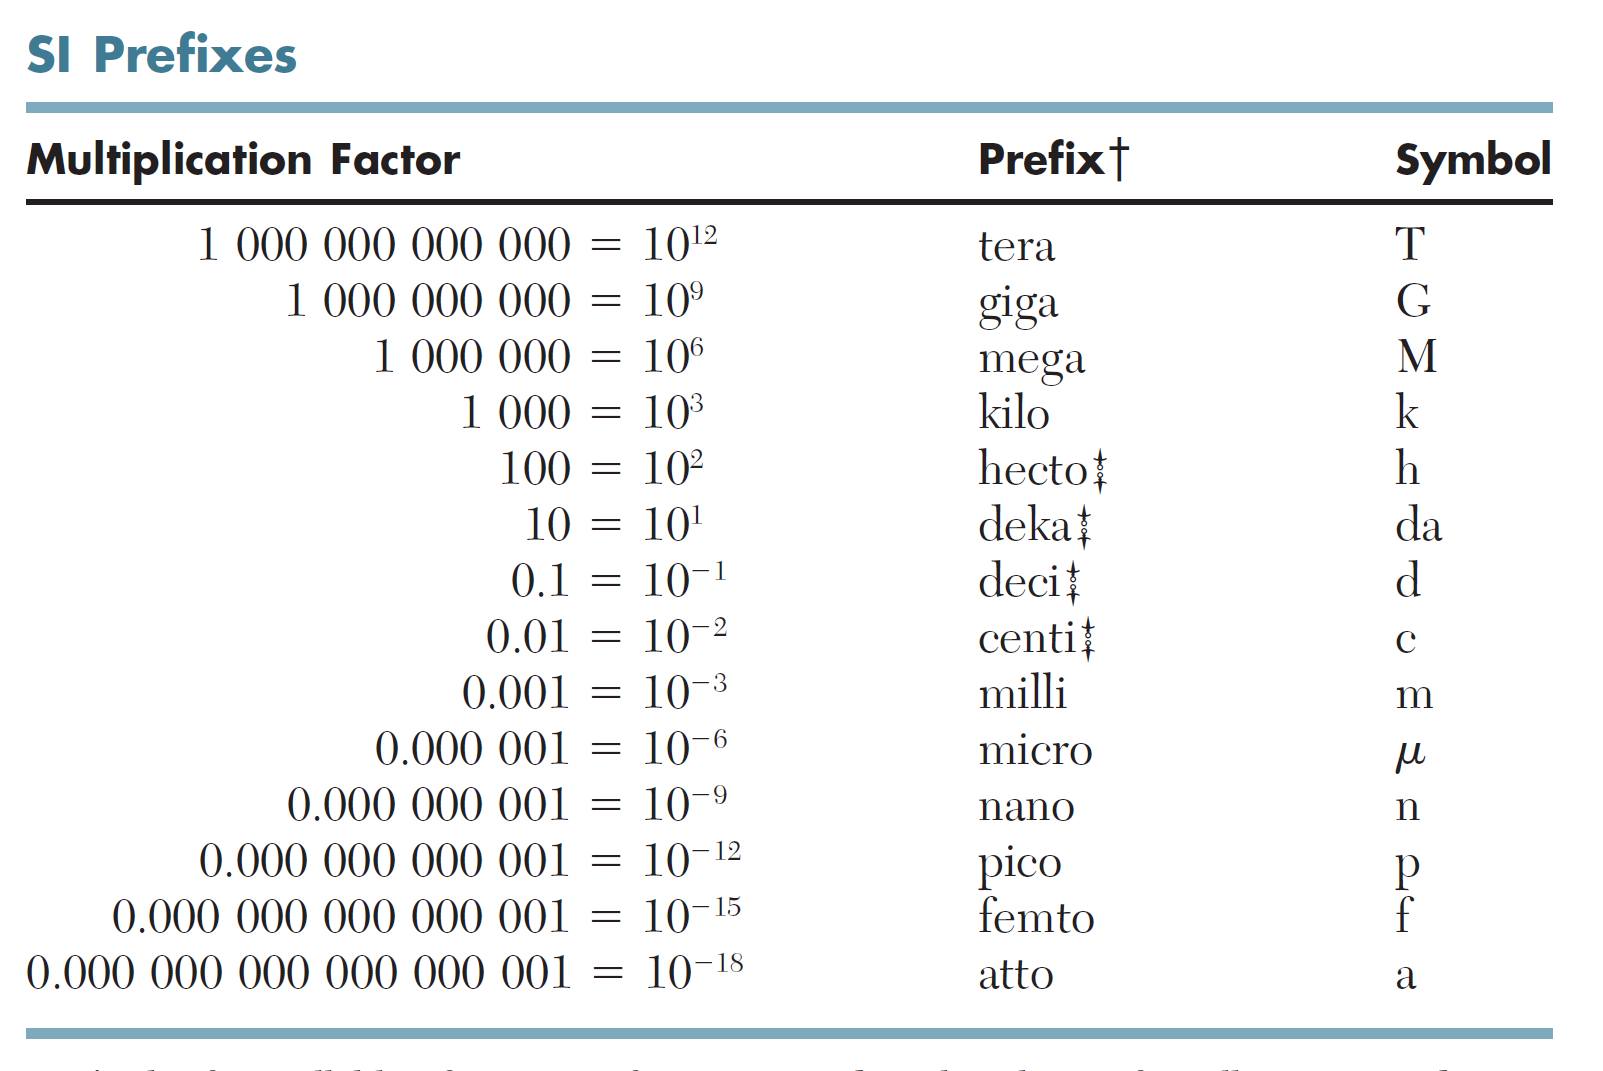
\includegraphics[width=\linewidth, height=8cm]{SI_Prefix.png}
\end{Figure}
% -----------------------------------------------------------------------
\section{Chapter 1 - Concept of stress}

\section{Chapter 2 - Stress and Strain - Axial Loading}

\section{Chapter 3 - Torsion}
\subsection{General}
\subsection{Deformation in Circular Shafts}
\begin{equation}
    \gamma=\frac{\rho\phi}{L}
\end{equation}
\begin{equation}
    \gamma_{max}=\frac{c\phi}{L}
\end{equation}
\begin{equation}
    \gamma=\frac{\rho}{c}*\gamma_{max}
\end{equation}
\subsection{Shearing Stresses in Elastic Range}
\begin{equation}
    \tau=\frac{\rho}{c}\tau_{max}
\end{equation}
\begin{equation}
    \tau_{max}=\frac{Tc}{J}
\end{equation}
\begin{equation}
    \tau=\frac{T\rho}{J}
\end{equation}
\subsubsection{Polar Moment of Inertia Solid Shaft}
\begin{equation}
    J=\frac{1}{2}\pi c^4
\end{equation}
c = radius
\subsubsection{Polar Moment of Inertia of a Hollow Shaft inner radius c1, outer radius c2}
\begin{equation}
    J=\frac{1}{2}\pi(c_2^4-c_2^4)
\end{equation}
\subsection{Angle of Twist}
\begin{equation}
    \phi=\frac{TL}{JG}
\end{equation}
\begin{equation}
    \phi=\Sigma\frac{TL}{JG}
\end{equation}
\subsection{Statically Indeterminante Shafts}
\subsection{Transmission Shafts}
Power P is transmitted as:
\begin{equation}
    P=2\pi fT
\end{equation}
T is the torque exerted at each end of the shaft\\*
f the frequency (hz or $s^{-1}$)
\subsection{Stress Concentrations}
\begin{equation}
    \tau_{\text{max}}=K\frac{Tc}{J}
\end{equation}
K = Stress concentration factor\\*
stress $\frac{Tc}{J}$ is computed for the smaller-diameter shaft
\begin{Figure}
    \centering
    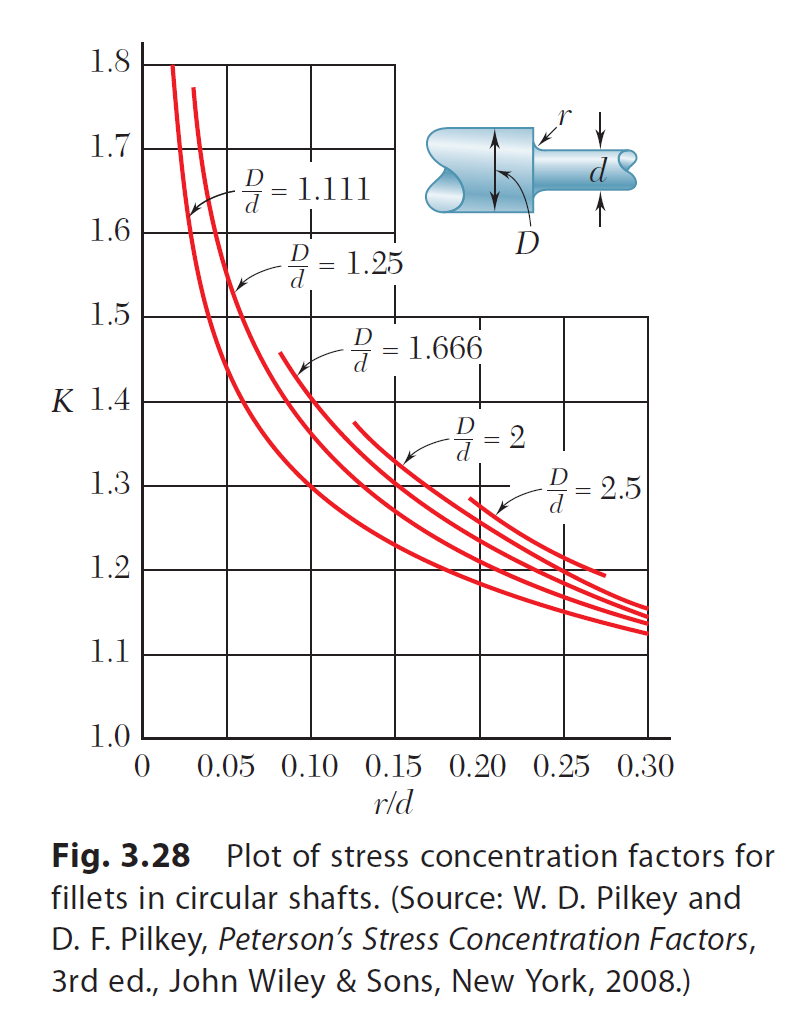
\includegraphics[width=\linewidth, height=8cm]{PlotStressConcentrationsFilletsRoundShaft.png}
\end{Figure}
\subsection{Plastic Deformations}
\begin{equation}
    T=\int^c_0\rho\tau(2\pi d\rho)=2\pi\int^c_0\rho^2\tau d\rho
\end{equation}
\subsection{Modulus of Rupture}
This is a ficticious value.
\begin{equation}
    R_t=\frac{T_uc}{j}
\end{equation}
\subsection{Solid Shaft of Elastoplastic Material}
\subsubsection{Maximum Elastic Torque; Solid Circular Shaft, Radius c}
\begin{equation}
    \tau_y=\frac{1}{2}\pi c^3\tau Y
\end{equation}
\subsubsection{Torque Related to $\rho_y$}
\begin{equation}
    T=\frac{4}{3}T_y(1-\frac{1}{4}\rho{\rho^3y}{c^3})
\end{equation}
\subsubsection{Plastic Torque}
\begin{equation}
    T_p=\frac{4}{3}T_y
\end{equation}
\subsubsection{Plastic Torque Vs. Angle of Twist}
\begin{equation}
    T=\frac{4}{3}T_y(1-\frac{1}{4}\frac{\phi^3y}{\phi^3})
\end{equation}
\subsubsection{Torsional Loading or Shaft Cross-Section Changes Along Length}
\begin{equation}
    \phi=\Sigma_i\frac{T_iL_i}{J_iG_i}
\end{equation}
\subsubsection{Thin-Walled Hollow Shafts}
\subsubsection{Shear Flow}
\begin{equation}
    q=\tau t
\end{equation}
\subsubsection{Average Shearing Stress $\tau$ at any given point in cross section}
\begin{equation}
    \tau=\frac{T}{2tA}
\end{equation}

% Example Figure
%\begin{Figure}
%    \centering
%    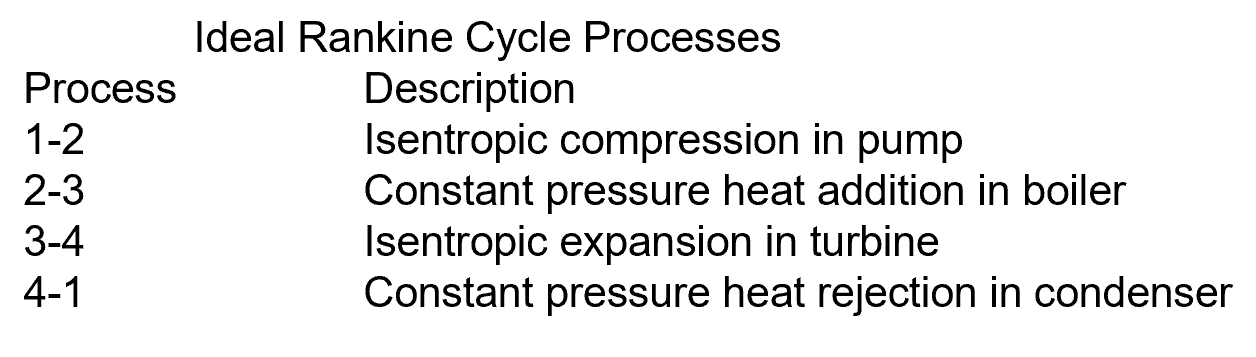
\includegraphics[width=\linewidth]{RankineCycleProcess.png}
%\end{Figure}

% References
%\rule{0.3\linewidth}{0.25pt}
%\scriptsize
%\bibliographystyle{abstract}
%\bibliography{Bibliography}

% End of document
\end{multicols}
\end{document}